\section{Exercícios}
\begin{frame}
\frametitle{Exercícios} 
\Ex{Na Definição 1 definimos seno e cosseno de um ângulo no
triângulo retângulo. Como você definiria, com os lados de um
triângulo retângulo, as demais relações trigonométricas da Definição
\ref{outrasfunctrig}?}

\Ex{Saber para quais valores $t$ são válidas algumas equações
envolvendo equações trigonométricas é muito importante. Determine o
conjunto solução de cada uma das equações abaixo:
\begin{enumerate}[(a)]
	\item $\sen t = 0$, $\cos t = 0$ e $\tan t = 0$;
	\item $\sen t = 1$, $\cos t = 1$;
	\item $\sen t = -1$, $\cos t = -1$ e $\tan t = -1$;
	\item $\sen t = \cos t$ e $\tan t = 1$;
	\item $\csc t = 0$, $\sec t = 0$ e $\cot t = 0$;
	\item $\csc t = 1$, $\sec t = 1$;
	\item $\csc t = -1$, $\sec t = -1$ e $\cot t = -1$;
	\item $\csc t = \sec t$ e $\cot t = 1$.
\end{enumerate}
}

\end{frame}


%------------------------------------------------------------------------------------------------------------

\begin{frame}
\frametitle{Exercícios} 


\Ex{A figura abaixo representa o gráfico da função $f_1 : \R \to
\R$, $f_1(x) = x \cdot \sen x$, traçado no intervalo $\colc{-20 \pi,
20 \pi}$, juntamente com as retas $y=x$ e $y=-x$.
\begin{center}
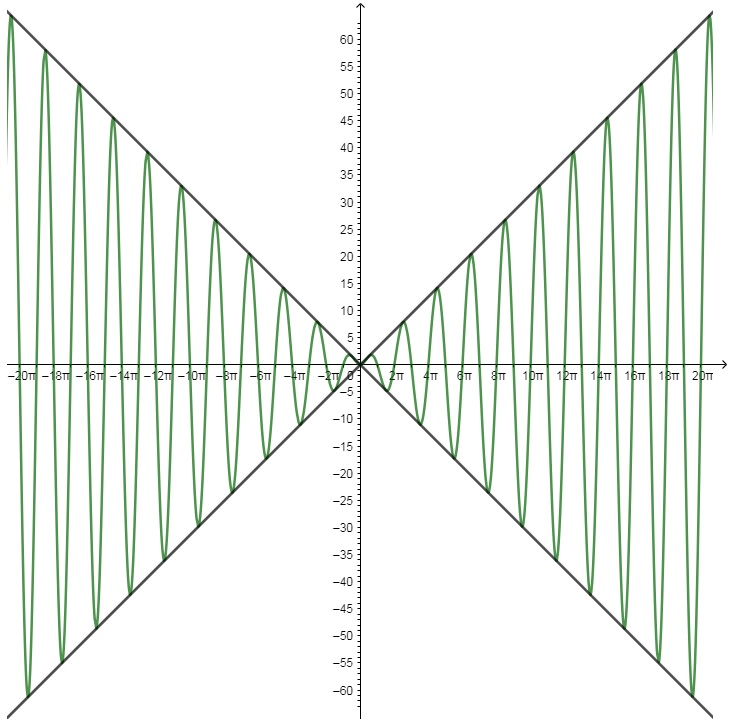
\includegraphics[width=2.5cm]{figures/grafxsenx.jpg}
\end{center}
\begin{enumerate}[(a)]
	\item Explique por que o gráfico de $f_1$ fica limitado entre
	essas retas e indique todos os pontos em que o gráfico toca as retas;
	\item Considere a seguinte afirmação: \emph{Os máximos e
	mínimos locais da função $f_1$ ocorrem nos mesmos valores
	de $x$ que os da função seno.} Esta afirmação é verdadeira?
	\item Como você espera visualizar o gráfico da função $f_2: \R \to
	\R$, definida por $f_2(x) = x^2 \cdot \sen x$?
\end{enumerate}}

\end{frame}

%------------------------------------------------------------------------------------------------------------

\begin{frame}
\frametitle{Exercícios} 

\Ex{Na figura abaixo, os segmentos $AD$ e $OD$ representam,
respectivamente, $\tan x$ e $\sec x$.
\begin{center}
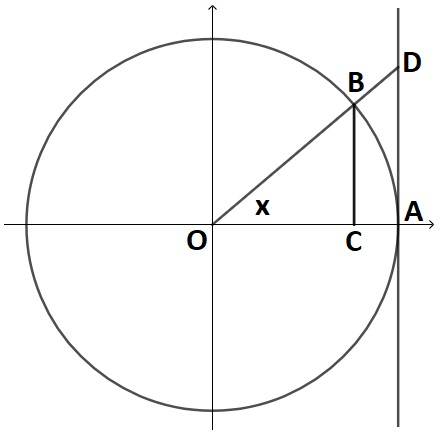
\includegraphics[width=4.5cm]{figures/circtansec.jpg}
\end{center}
\begin{enumerate}[(a)]
	\item Justifique a afirmação acima;
	\item Qual a interpretação dos sinais de $\tan x$ e $\sec x$ na
	figura?
	\item Faça uma figura análoga para representar $\cot x$ e $\csc
	x$, justificando a construção.
\end{enumerate}}


\end{frame}


%------------------------------------------------------------------------------------------------------------

\begin{frame}
\frametitle{Exercícios} 

\Ex{Encontre as três menores soluções positivas da equação $$\cos
\paren{3x - \frac {\pi} 4} = 0.$$}

\begin{exercise}
	Sem utilizar as fórmulas de seno e cosseno da soma de dois arcos,
	mostre que, para todo $t\in\reals$, vale \[\cos\prn{\frac \pi 2-t}=\sen t\]
\end{exercise}
  
\begin{exercise}
	Um triângulo tem um de seus lados medindo $\sqrt{3}-1$ e seu ângulo oposto medindo $\dfrac{\pi}{6}$. Dado que outro ângulo do triângulo mede $\dfrac{\pi}{4}$, qual a medida do maior de seus lados?
\end{exercise}
  
\begin{exercise}
	Considere um triângulo retângulo tal que seu perímetro é igual a $\dfrac{\raiz 6 + 2}{2}$ e sua hipotenusa mede $1$. Calcule a medida do menor de seus ângulos.
\end{exercise}

\end{frame}


%------------------------------------------------------------------------------------------------------------

\begin{frame}
\frametitle{Exercícios} 
  
\begin{exercise}
	Um triângulo $ABC$ possui lados que medem $a=10$, $b = 12$ e $c=8$, onde o lado $a$ é oposto ao ângulo $\hat A$, $b$ ao $\hat B$ e $c$ ao $\hat C$. Mostre que $\hat B = 2\hat C$.
\end{exercise}

\Ex{Mostre que o perímetro do pentágono regular inscrito em um
círculo unitário é dado por $10\sen \frac {\pi} 5$.}

\Ex{Considere a função $f: \R \to \R$ definida por $f(x) = \sen
\paren{ax}+\sen \paren{bx}$, em que $a$ e $b$ são constantes reais.
\begin{enumerate}[(a)]
	\item Mostre que, se $a$ e $b$ são racionais, então $f$ é
	periódica;\\
	\emph{Dica:} Mostre que o período de $\sen \paren{ax}$ é $\frac
	{2\pi} a$.
	\item A recíproca da afirmação do item anterior é verdadeira?
	Justifique sua resposta.
\end{enumerate}}

\Ex{
	Considere a função trigonométrica $f(x) = \sen x$.
        \begin{enumerate}[a)]
            \item  Com ajuda do círculo trigonométrico, escreva um intervalo onde $f$ é crescente e possua os valores onde $f$ atinge seu máximo e mínimo absolutos.
            \item  Generalize o intervalo de crescimento do item anterior para cada $k \in \Z$.
        \end{enumerate}
}

\end{frame}



%------------------------------------------------------------------------------------------------------------


\begin{frame}
\frametitle{Exercícios} 

\Ex{Prove as identidades abaixo, válidas para todo $x$ onde as
expressões estão definidas:
\begin{enumerate}[(a)]
	\item $\dfrac{1-\tan^2 x}{1+\tan^2 x} = 1 - 2\sen^2 x$;
  \item $\dfrac{\cos x - \sen x}{\cos x + \sen x} = \dfrac{1 - \tan x}{1+\tan
  x}$;
  \item $\dfrac{\sen x}{\csc x - \cot x} = 1+ \cos x$;
  \item $\cos^2 x = \frac {1+\cos \paren{2x}} 2$;
  \item $\sen^2 x = \frac {1-\cos \paren{2x}} 2$;
  \item $\sen(mx)\cdot\cos(nx)=\dfrac{\sen[(m-n)x]+\sen[(m+n)x]}{2}$;
  \item $\sen(mx)\cdot\sen(nx)=\dfrac{\cos[(m-n)x]-\cos[(m+n)x]}{2}$;
  \item $\dfrac{1-\tan^2 x}{1+\tan^2 x} = \cos^2 x - \sen^2 x = \cos \paren{2x}$;
  \item $\dfrac{2\tan x}{1+\tan^2 x} = 2\sen x \cos x= \sen\paren{2x}$.
\end{enumerate}}

\end{frame}



%------------------------------------------------------------------------------------------------------------

\begin{frame}
\frametitle{Exercícios} 

\Ex{
    Considere $x \in \R$ tal que $3{,}5 < x < 6$.
    Calcule o conjunto solução da inequação $-2 \cos^2 x + \sen x + 1 \geq 0$.
}

\Ex{
    Considere $x \in \R$ tal que $2 < x < 4$.
    Calcule o conjunto solução da equação $\sec^2 x + \dfrac{2 \sqrt 3}{3} \tan x = 2$.
}

\Ex{Use as fórmulas de seno e cosseno da soma para determinar os
senos e cossenos dos seguintes ângulos (medidos em radianos): $\dfrac
{\pi} 8$, $\dfrac{\pi} {12}$, $\dfrac {3\pi} 8$ e $\dfrac{5\pi}{12}$.}

\Ex{
	Considere as funções seno e cosseno definidas em $\R$. 
            \begin{enumerate}[a)]
	       \item  Prove, para todo $t \in \R$, a identidade $\cos t = \sen \left(\dfrac \pi 2 - t \right)$ sem utilizar o círculo trigonométrico.
	       \item Considere que o gráfico da função seno é conhecido. Como você poderia obter o gráfico da função cosseno mediante a identidade anterior?
			\end{enumerate}
}

\end{frame}


%------------------------------------------------------------------------------------------------------------

\begin{frame}
\frametitle{Exercícios} 

\begin{exercise}
	Considere dois ângulos $\alpha$ e $\beta$, tais que $0 < \alpha < \dfrac \pi 2$ e $0 < \beta < \dfrac \pi 2$. Na figura abaixo temos um círculo trigonométrico, onde são marcados os pontos $A$, $B$, $C$ e $D$ de tal sorte que $\alpha = \widehat{AOB}$ e $\beta = \widehat{BOC} = \widehat{AOD}$.
	\begin{figure}[H]
		\centering
	  \importtikz{exercicio-cos_da_soma}
	  \label{fig:cos-da-soma}
	\end{figure}
\end{exercise}

\end{frame}


%------------------------------------------------------------------------------------------------------------

\begin{frame}
\frametitle{Exercícios} 
	\begin{enumerate}[a)]
	  \item Utilizando os conceitos de trigonometria, escreva as coordenadas dos pontos $A$, $B$, $C$ e $D$;
	  \item Determine $\overline{AC}$ (medida do comprimento do segmento $AC$) em função das coordenadas de $A$ e $C$;
	  \item Determine $\overline{BD}$ em função das coordenadas de $B$ e $D$;
	  \item Sabendo que $\overline{AC} = \overline{BD}$, use os itens anteriores para mostrar a fórmula para $\cos (\alpha + \beta)$.
	\end{enumerate}
  
  
\begin{exercise}
	Considere dois ângulos $\alpha$ e $\beta$, tais que $0 < \alpha < 2 \pi$, $0 < \beta < 2 \pi$ e $\alpha > \beta$. Nas figuras dos próximos slides temos um círculo trigonométrico, onde são marcados os pontos $A$, $B$ e $C$ de tal sorte que $\alpha = \widehat{AOC}$ e $\beta = \widehat{AOB}$ em dois casos distintos. Quando $\alpha - \beta < \pi$ (Caso 1) e $\pi < \alpha - \beta < 2\pi$ (Caso 2). 
\end{exercise}

\end{frame}


%------------------------------------------------------------------------------------------------------------

\begin{frame}
\frametitle{Exercícios} 
	\begin{figure}[H]
	  \centering
	  \importtikz{exercicio-cos-da-diferenca1}
	  \caption{Caso 1.}
	  \label{fig:cos-da-diferenca1}
	\end{figure}

\end{frame}


%------------------------------------------------------------------------------------------------------------

\begin{frame}
\frametitle{Exercícios} 
  
	\begin{figure}[H]
	  \centering
	  \importtikz{exercicio-cos-da-diferenca2}
	  \label{fig:cos-da-diferenca2}
	  \caption{Caso 2.}
	\end{figure}

\end{frame}


%------------------------------------------------------------------------------------------------------------

\begin{frame}
\frametitle{Exercícios} 
  
	\textit{Observação}: para as resoluções abaixo, não podem ser utilizadas as fórmulas das funções trigonométricas de adição e subtração de arcos.
	\begin{enumerate}[a)]
		\item Utilizando os conceitos de trigonometria, escreva as coordenadas dos pontos $B$ e $C$ de modo que sirvam para ambos os casos;
		\item Utilize o triângulo $OBC$ do Caso 1 para demonstrar a fórmula do cosseno da diferença de dois arcos, ou seja, para $\cos (\alpha - \beta)$;
		\item  Utilize o triângulo $OBC$ do Caso 2 para demonstrar a fórmula do cosseno da diferença de dois arcos, ou seja, para $\cos (\alpha - \beta)$.
  \end{enumerate}
  
  
  \begin{exercise}
	  Obtenha fórmulas para: 
	  \begin{enumerate}[a)]
		\item $\tan\paren{\alpha + \beta}$ em função de $\tan \alpha$ e $\tan \beta$;
		\item $\tan\paren{\alpha - \beta}$ em função de $\tan \alpha$ e $\tan \beta$;
		\item $\tan\paren{2 \alpha}$ em função de $\tan \alpha$;
		\item $\sec \paren{\alpha + \beta}$ em função de $\sec \alpha$, $\sec \beta$, $\tan \alpha$ e $\tan \beta$.
	  \end{enumerate}
  \end{exercise}

\end{frame}


%------------------------------------------------------------------------------------------------------------

\begin{frame}
\frametitle{Exercícios} 
  
\begin{exercise}
	Pedro afirma que, em competições de tiro, acertar um alvo na diagonal é mais difícil do que acertar um alvo que está à frente por conta que o ângulo de visão do alvo na diagonal é menor. A figura no próximo slide (fora de escala) simula uma situação em uma competição de tiros, onde Pedro está no ponto P a 25m de distância do alvo à frente, cada alvo tem 0,5m de diâmetro e distam 4,75m um do outro.
\end{exercise}

\end{frame}


%------------------------------------------------------------------------------------------------------------

\begin{frame}
\frametitle{Exercícios} 

		  \begin{figure}[H]
			\centering 
			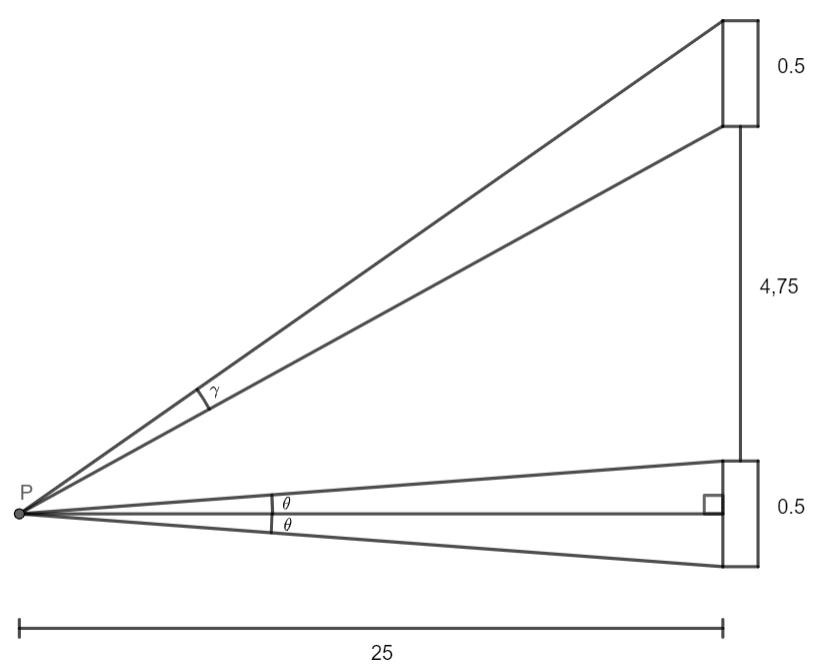
\includegraphics[width=7cm]{figures/exercicio-angulos-de-visao.png} 
			%\caption{Ângulos de visão dos alvos.}
			\label{fig:angulos-de-visao}
		  \end{figure}
		  Com a notação da figura, mostre que o ângulo de visão do alvo na diagonal é menor que o ângulo de visão do alvo à frente, ou seja, $\gamma < 2\theta$. Para tanto, use o conceito de tangente no triângulo retângulo e o fato de tangente ser uma função crescente. %É permitido o uso de uma calculadora para contas básicas de soma, multiplicação e divisão.
  

\end{frame}

%------------------------------------------------------------------------------------------------------------